\section{Numerical studies}
\iffalse %(1)
\subsection{Simulation}
\begin{frame}{Simulation}
비교 모델
\begin{itemize}
\item Regression Spline (RS)

보조변수 (auxiliary variable) 없이 B-spline basis의 선형 적합
\item Smoothing Spline (SS)

모든 예측변수에 대해 매듭 지정, smoothing 과 shrinkage 적용
\item Local Regression (LR) and Local Polynomial (LP)

 moving average, polynomial regression
\item 평가 기준 : MSE, MAE
$$
MSE(\hat{f}) = \frac{1}{n} \sum_{i = 1}^n (\hat{f}(x_i) - f(x_i))^2
\quad \mbox{and} \quad
MAE(\hat{f}) = \frac{1}{n} \sum_{i = 1}^n |\hat{f}(x_i) - f(x_i)|
$$
\end{itemize}
\end{frame}

\begin{frame}{Simulation -  Underlying function}
\begin{figure}
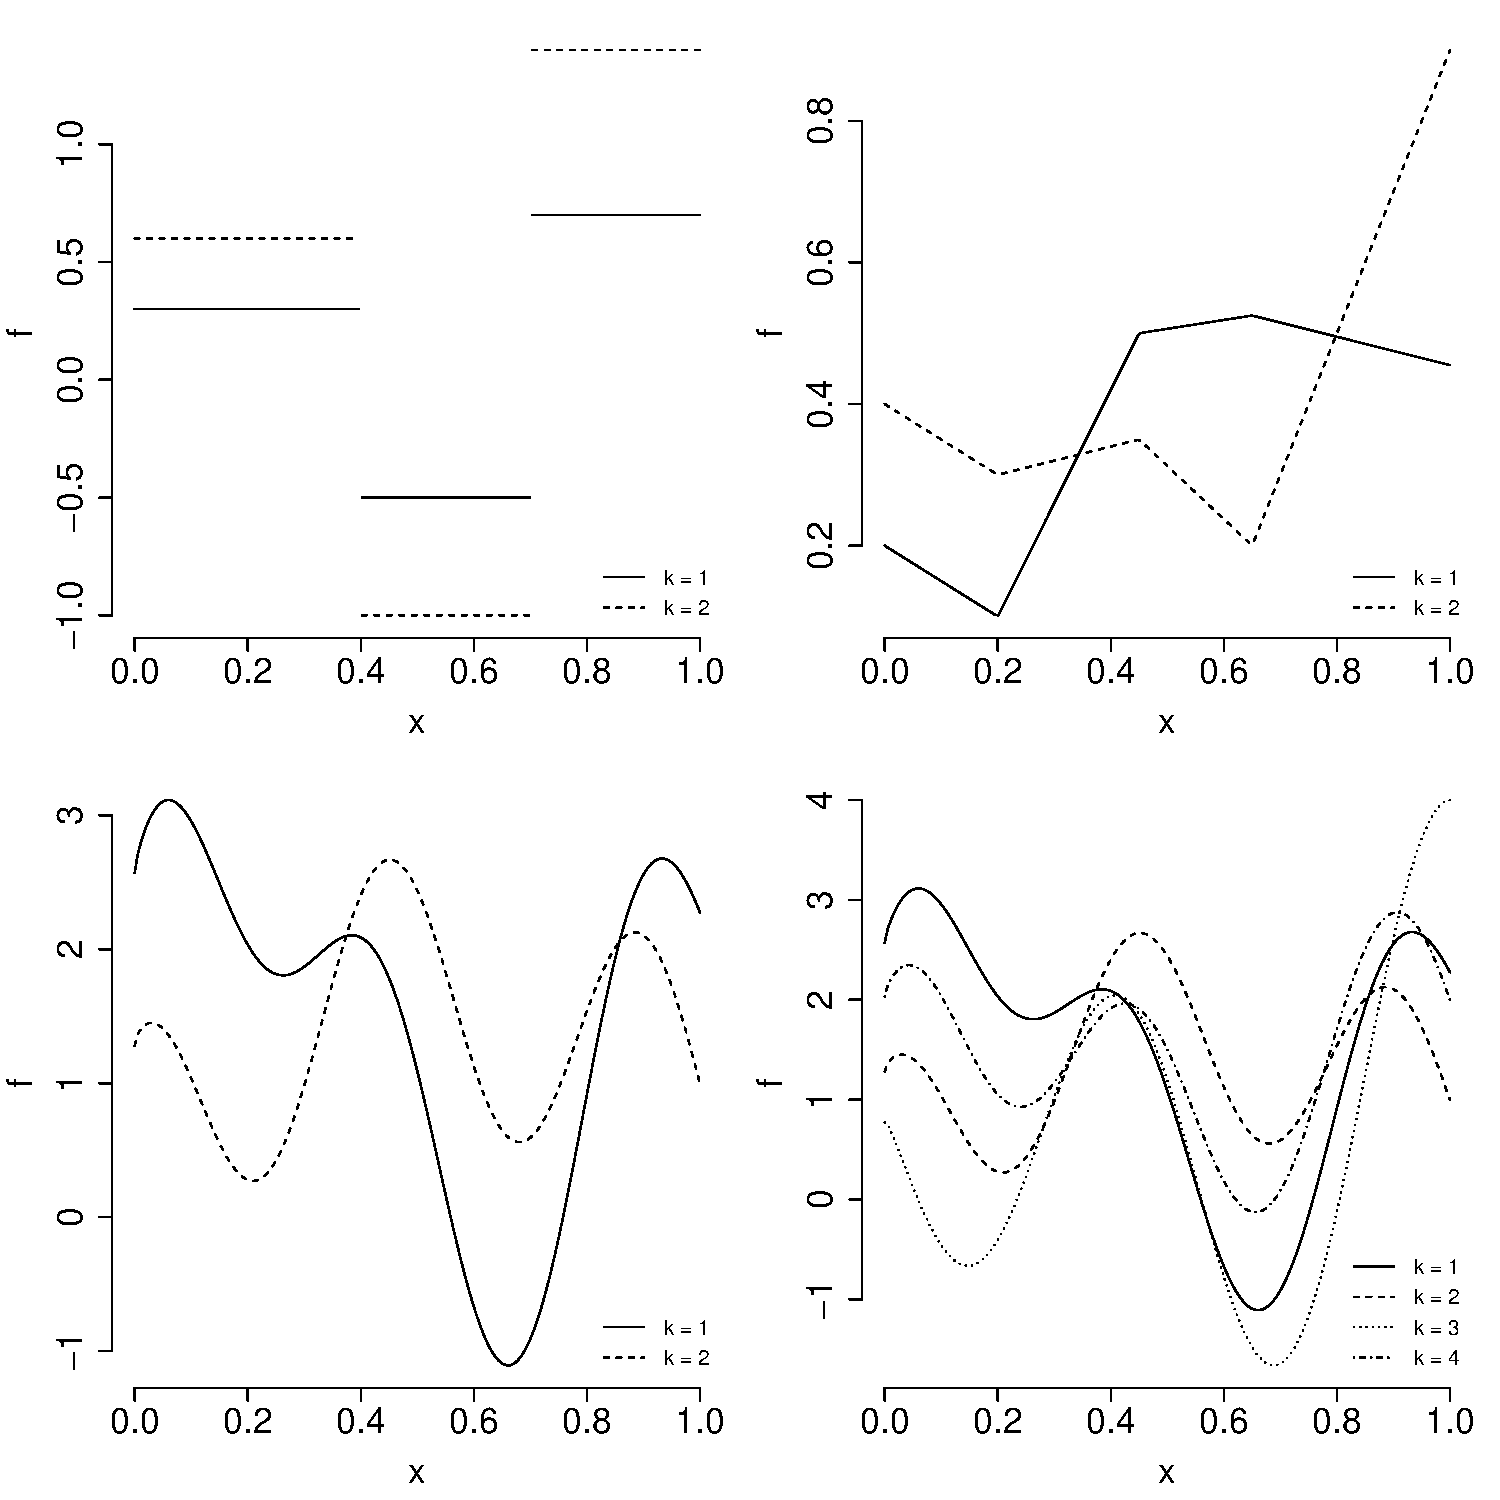
\includegraphics[scale = 0.28]{true_function}
\end{figure}
\end{frame}

\begin{frame}{Simulation - Results}
\begin{table}[!htb]
\centering
\footnotesize
\caption{The average of each criterion ($\times 100$) over $100$ runs of OUR, RS,
SS, LR, and LP for Example 1 with a sample size $n = 200, 500$ and a signal-to-noise ratio 
$SNR = 5, 15$, with the standard error in parentheses. The bold text is the smallest
criterion in each scenario.}
\label{tb : ex1}
\tabcolsep=5pt
\begin{tabular}{lllll||lllll}
  \hline
$n$ & SNR & Method & MSE & MAE & $n$ & SNR & Method & MSE & MAE \\ 
  \hline
200 & 5 & PSE & \textbf{2.86(1e-03)} & \textbf{8.77(2e-03)} & 500 & 5 & PSE & \textbf{2.13(5e-04)} & \textbf{5.88(1e-03)} \\ 
   &  & RS & 8.96(6e-04) & 25.29(8e-04) &  &  & RS & 8.31(3e-04) & 25.20(3e-04) \\ 
   &  & SS & 4.02(7e-04) & 13.96(1e-03) &  &  & SS & 2.52(3e-04) & 10.65(1e-03) \\ 
   &  & LR & 13.93(1e-03) & 26.07(1e-03) &  &  & LR & 14.10(8e-04) & 26.01(8e-04) \\ 
   &  & LP & 11.86(8e-03) & 18.16(4e-03) &  &  & LP & 6.57(3e-03) & 12.54(2e-03) \\  \cline{2-5} \cline{7-10}
   & 15 & PSE & \textbf{1.79(7e-04)} & \textbf{5.52(1e-03)} &  & 15 & PSE & 1.68(5e-04) & \textbf{3.83(7e-04)} \\ 
   &  & RS & 8.34(6e-04) & 25.20(6e-04) &  &  & RS & 8.06(3e-04) & 25.16(3e-04) \\ 
   &  & SS & 2.15(4e-04) & 9.57(8e-04) &  &  & SS & \textbf{1.35(2e-04)} & 7.48(5e-04) \\ 
   &  & LR & 13.72(1e-03) & 25.47(1e-03) &  &  & LR & 13.74(8e-04) & 25.40(7e-04) \\ 
   &  & LP & 9.58(7e-03) & 13.98(4e-03) &  &  & LP & 6.11(3e-03) & 9.78(2e-03) \\ 
   \hline
\end{tabular}
\end{table}
\end{frame}

\begin{frame}{Simulation - Results}

\end{frame}
\fi %(1)

\subsection{Real data}
\begin{frame}{Bone mineral density data}
\begin{itemize}
\item 성별에 따라 골밀도의 분포가 다름
\end{itemize}
\begin{figure}
\includegraphics[scale=0.35]{BMD}
\end{figure}
\end{frame}

\begin{frame}{Bone mineral density data}
\begin{itemize}
\item 인종에 따라 골밀도의 분포가 다름
\end{itemize}
\begin{figure}
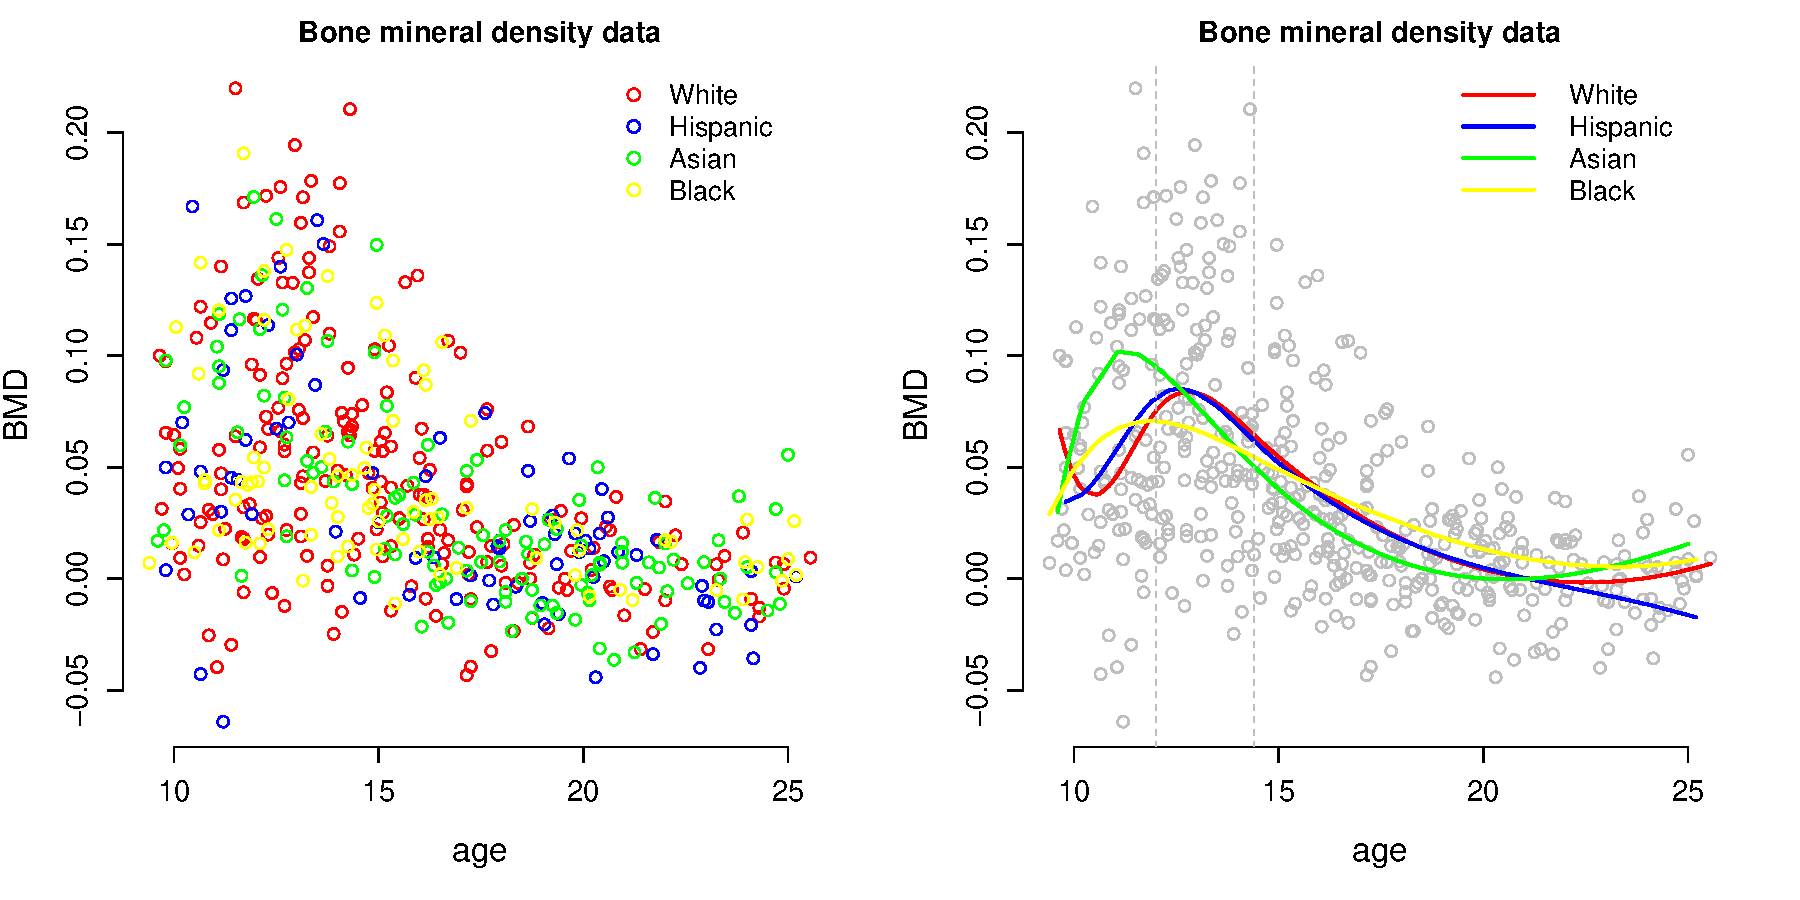
\includegraphics[scale=0.35]{BMD_e}
\end{figure}
\end{frame}

\begin{frame}
\begin{figure}
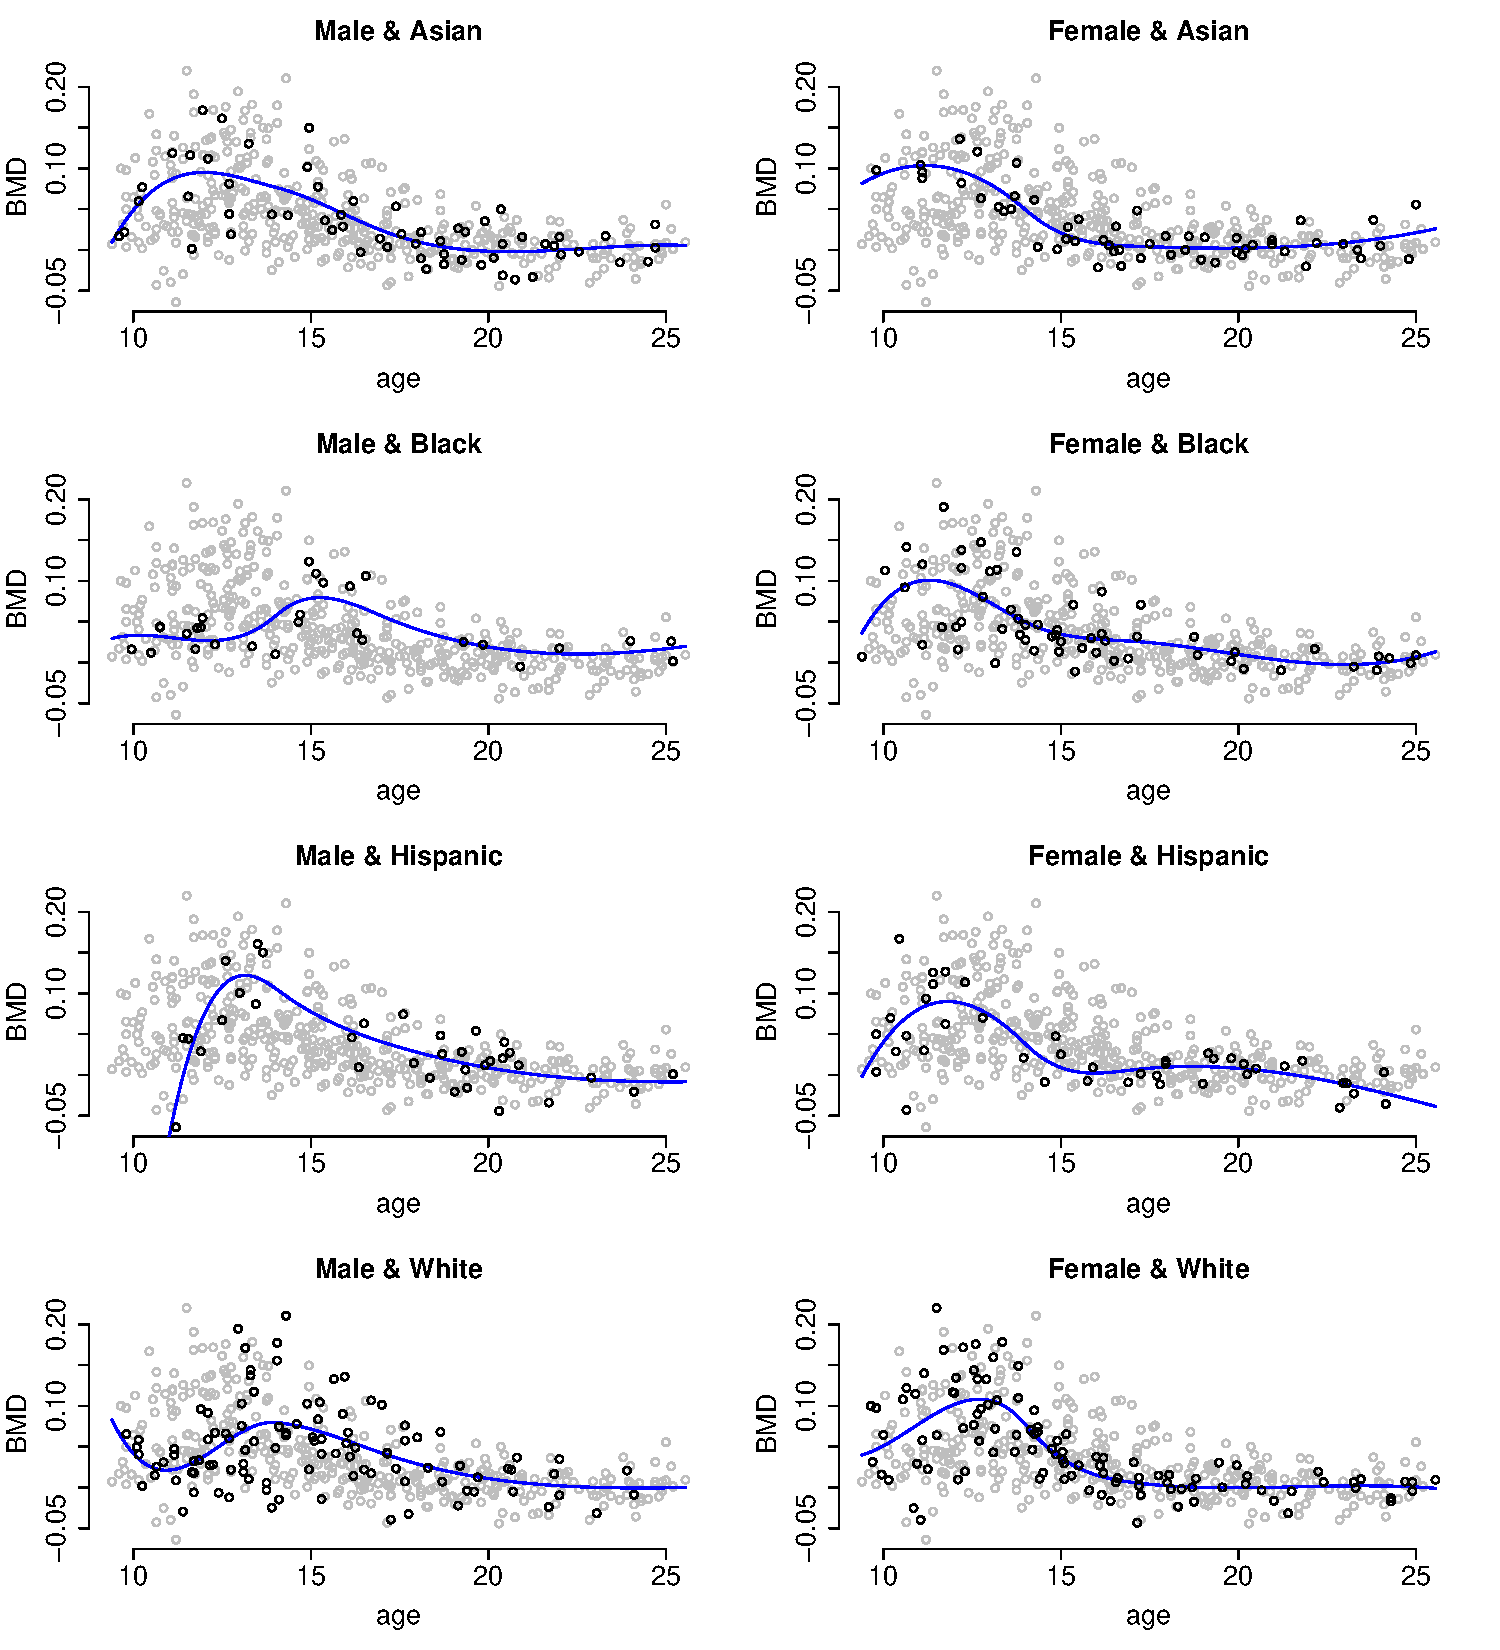
\includegraphics[scale=0.3]{gridz8_blue}
\end{figure}
\end{frame}
